%%%%%%%%%%%%%%%%%%%%%%%%%%%%%%%%%%%%%%%%%%%%%%%%%%%%%%%%%%%%%%%
%
% Welcome to Overleaf --- just edit your LaTeX on the left,
% and we'll compile it for you on the right. If you open the
% 'Share' menu, you can invite other users to edit at the same
% time. See www.overleaf.com/learn for more info. Enjoy!
%
%%%%%%%%%%%%%%%%%%%%%%%%%%%%%%%%%%%%%%%%%%%%%%%%%%%%%%%%%%%%%%%
% --------------------------------------------------------------
% Homework Template by Dana Ernst, reproduced here with thanks.
% --------------------------------------------------------------
% This is all preamble stuff that you don't have to worry about.
% Head down to where it says "Start here"
% --------------------------------------------------------------

\documentclass[12pt]{article}
\usepackage{titlesec}

\usepackage[margin=1in]{geometry} 
\usepackage{amsmath,amsthm,amssymb}
\usepackage{cite}
\usepackage{graphicx}

\newcommand{\N}{\mathbb{N}}
\newcommand{\Z}{\mathbb{Z}}

\newcommand{\Eqref}[1]{Eq.~\eqref{#1}}
\newcommand{\Figref}[1]{Fig.~\ref{#1}}

% this improves readability of to-do notes
\setlength{\marginparwidth}{2.20cm}
\usepackage[color=green!60]{todonotes}
\newcommand{\tde}[1]{\todo[color=blue!20]{\footnotesize #1 \\--ECD}}
\newcommand{\tdei}[1]{\todo[inline,color=blue!20]{\footnotesize #1 --ECD}}

\newenvironment{theorem}[2][Theorem]{\begin{trivlist}
\item[\hskip \labelsep {\bfseries #1}\hskip \labelsep {\bfseries #2.}]}{\end{trivlist}}
\newenvironment{lemma}[2][Lemma]{\begin{trivlist}
\item[\hskip \labelsep {\bfseries #1}\hskip \labelsep {\bfseries #2.}]}{\end{trivlist}}
\newenvironment{exercise}[2][Exercise]{\begin{trivlist}
\item[\hskip \labelsep {\bfseries #1}\hskip \labelsep {\bfseries #2.}]}{\end{trivlist}}
\newenvironment{problem}[2][Problem]{\begin{trivlist}
\item[\hskip \labelsep {\bfseries #1}\hskip \labelsep {\bfseries #2.}]}{\end{trivlist}}
\newenvironment{question}[2][Question]{\begin{trivlist}
\item[\hskip \labelsep {\bfseries #1}\hskip \labelsep {\bfseries #2.}]}{\end{trivlist}}
\newenvironment{corollary}[2][Corollary]{\begin{trivlist}
\item[\hskip \labelsep {\bfseries #1}\hskip \labelsep {\bfseries #2.}]}{\end{trivlist}}

\begin{document}

% --------------------------------------------------------------
%                         Start here
% --------------------------------------------------------------

\title{Autocorrelation times and dynamical critical exponents in CRBM's}%replace X with the appropriate number
\author{Emanuel Casiano-Diaz}
\maketitle

Motivated by Fig 3(b) of \cite{Alcalde_Puente_2020}, we were interested in computing the integrated autocorrelation time of Ising model observables as a function of linear size near criticality. From this, one could then compare the dynamical critical exponent $z$ obtained from observables sampled via CRBM/Gibbs with observables sampled with Metropolis-Hastings. Moreover, how does the autocorrelation time scale away from the critical temperature?

% --------------------------------------------------------------
\section*{Dynamical critical exponent}

The dynamical critical exponent in the nearest-neighbor 2D Ising model is known to be $z \approx 2.1$. Fig 3(b) of \cite{Alcalde_Puente_2020} seems to suggest that $z$ differs considerably when sampling with the CRBM vs sampling with Metropolis-Hastings.

\Figref{fig:tau_M_Tc} shows the autocorrelation time of the magnetization near the critical temperature ($T_c\approx2.7$). For the CRBM, the dynamical critical exponent was estimated to be $z \approx 2.10 \pm 0.03$, whereas for Metropolis, it was $z \approx 2.14 \pm 0.03$. So both estimates are the same, within error bars. 

Even though the dynamical critical exponent for both methods is the same, it seems surprising that the autocorrelation time for the CRBM is larger than for Metropolis. In the \cite{Alcalde_Puente_2020}, results are shown that indicate that as systems get larger, the CRBM should yield much less correlation between samples.

This might be due to the way that samples were measured in their case vs how I collected them. In my case, I measured Metropolis samples every single time that at least $L^2$ spin flips were proposed. In their case, they collect samples every time that $k$ spin flips have been proposed, where $k$ is the number of spin flips that can be performed for each single Gibbs step of the CRBM. This number will vary depending on the system size.

%%%%%%%%%%%%%%%%%%%%%%%%%%%%%%%%%%%%%%%%%%%%%%%%%%
\begin{figure}[t!]
\begin{center}
    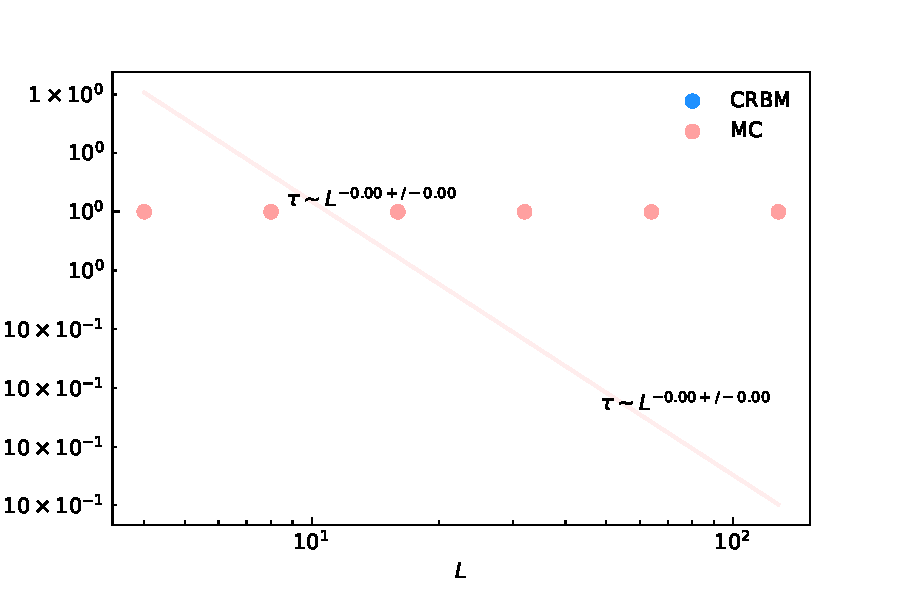
\includegraphics[width=1.0\columnwidth]{../figures/L_many_T_2.27_J1_-1.0_J2_0.0_seed_1968_kernelDims_2-2_analytical_autocorr_M.pdf}
\end{center}
\caption{Autocorrelation time of magnetization at $T_c\approx2.27$ as a function of linear size. Dynamical critical exponents are shown for CRBM and Metropolis.}
\label{fig:tau_M_Tc}
\end{figure}
%%%%%%%%%%%%%%%%%%%%%%%%%%%%%%%%%%%%%%%%%%%%%%%%%%

%%%%%%%%%%%%%%%%%%%%%%%%%%%%%%%%%%%%%%%%%%%%%%%%%%
%\begin{figure}[t!]
%\begin{center}
%    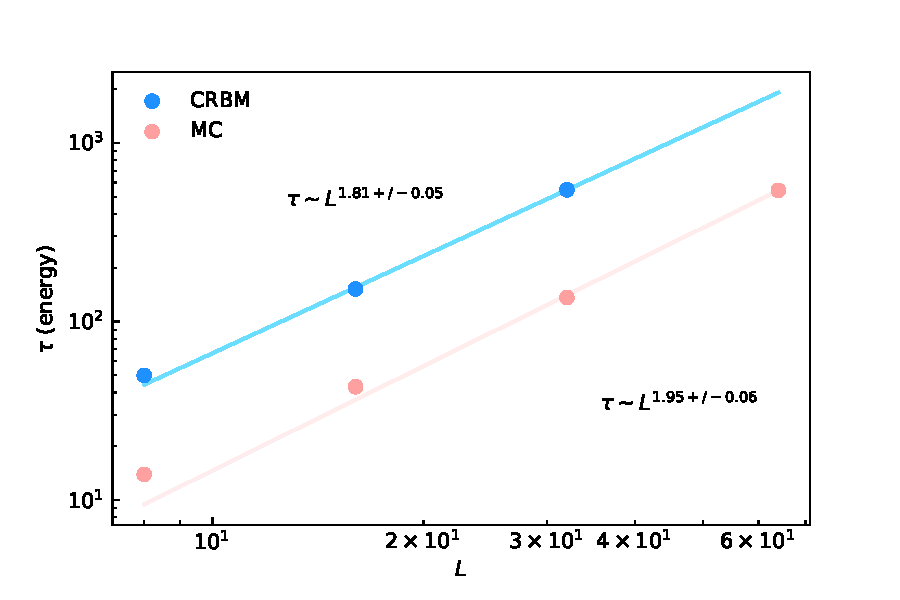
\includegraphics[width=1.0\columnwidth]{../figures/L_many_T_2.27_J1_-1.0_J2_0.0_seed_1968_kernelDims_2-2_analytical_autocorr_E.pdf}
%\end{center}
%\caption{Heatmap of learned kernels. The top two kernels show the learned weights for the case in which the CRBM was trained using the original data set. The bottom kernel corresponds to the case of the rotated data set. The colors seem to suggest that the learned weights in both cases were roughly the same, with the only difference being that the top-right and bottom-left weights are swapped.}
%\label{fig:2by2_kernels_heatmap}
%\end{figure}
%%%%%%%%%%%%%%%%%%%%%%%%%%%%%%%%%%%%%%%%%%%%%%%%%%

\section*{Autocorrelation times away from $T_c$}

To try and replicate figure 3(a) from \cite{Alcalde_Puente_2020}, and a similar other from Alcalde's thesis, I now compute the autocorrelation time away from $T_c$ and sampling Metropolis observables only every other $k$ steps. A table of $k$ values for various systems sizes can be seen in an appendix of \cite{Alcalde_Puente_2020}.

\Figref{fig:tau_E_2.2} and \Figref{fig:tau_E_2.4} show the autocorrelation time of the energy as functions of $L$, for temperatures $T=2.2$ and $T=2.4$, respectively. Notice that using their sampling, we see that for $L>100$, the CRBM outperforms Metropolis.

Should one then compare the critical exponents using this sampling?

%%%%%%%%%%%%%%%%%%%%%%%%%%%%%%%%%%%%%%%%%%%%%%%%%%
\begin{figure}[h!]
\begin{center}
    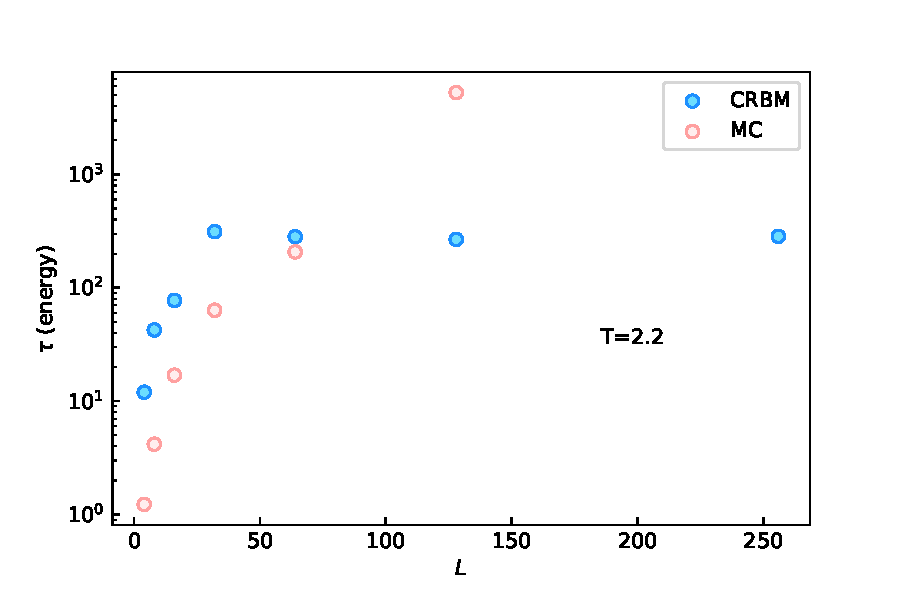
\includegraphics[width=1.0\columnwidth]{../figures/L_many_T_2.2_J1_-1.0_J2_0.0_seed_1968_kernelDims_2-2_analytical_autocorr_E.pdf}
\end{center}
\caption{Autocorrelation time of the energy at $T=2.2$ as a function of $L$.}
\label{fig:tau_E_2.2}
\end{figure}
%%%%%%%%%%%%%%%%%%%%%%%%%%%%%%%%%%%%%%%%%%%%%%%%%%

%%%%%%%%%%%%%%%%%%%%%%%%%%%%%%%%%%%%%%%%%%%%%%%%%%
\begin{figure}[h!]
\begin{center}
    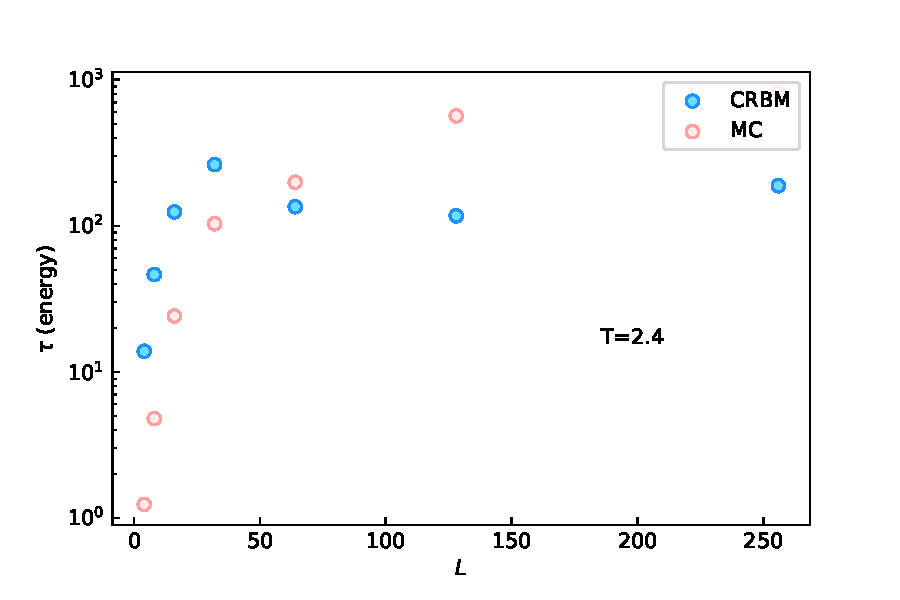
\includegraphics[width=1.0\columnwidth]{../figures/L_many_T_2.4_J1_-1.0_J2_0.0_seed_1968_kernelDims_2-2_analytical_autocorr_E.pdf}
\end{center}
\caption{Autocorrelation time of the energy at $T=2.4$ as a function of $L$.}
\label{fig:tau_E_2.4}
\end{figure}
%%%%%%%%%%%%%%%%%%%%%%%%%%%%%%%%%%%%%%%%%%%%%%%%%%

% --------------------------------------------------------------
%\newcommand{\sectionbreak}{\clearpage}
%\section{Test: Free-energy for non-symmetrized vs symmetrized kernels}

% --------------------------------------------------------------

\bibliographystyle{plain}
\bibliography{refs}

\end{document}